\documentclass[../Paper.tex]{subfiles}

\begin{document}
\section{Realization}

1. The calculation of pressure received by solar sail  

Hypothesis:

1)The energy emitted by the solar unit time is constant; 

2)The radiant energy absorbed by mercury, Venus, and the earth is negligible; 

3)Only consider in the solar system. 

According to the three hypothesis above, by conversation of energy:

\[S.\dfrac{4}{3}\pi{R_E}^2=S.(rdfrac{4}{3}\pi r^2\]






\begin{figure}[H]
\centering
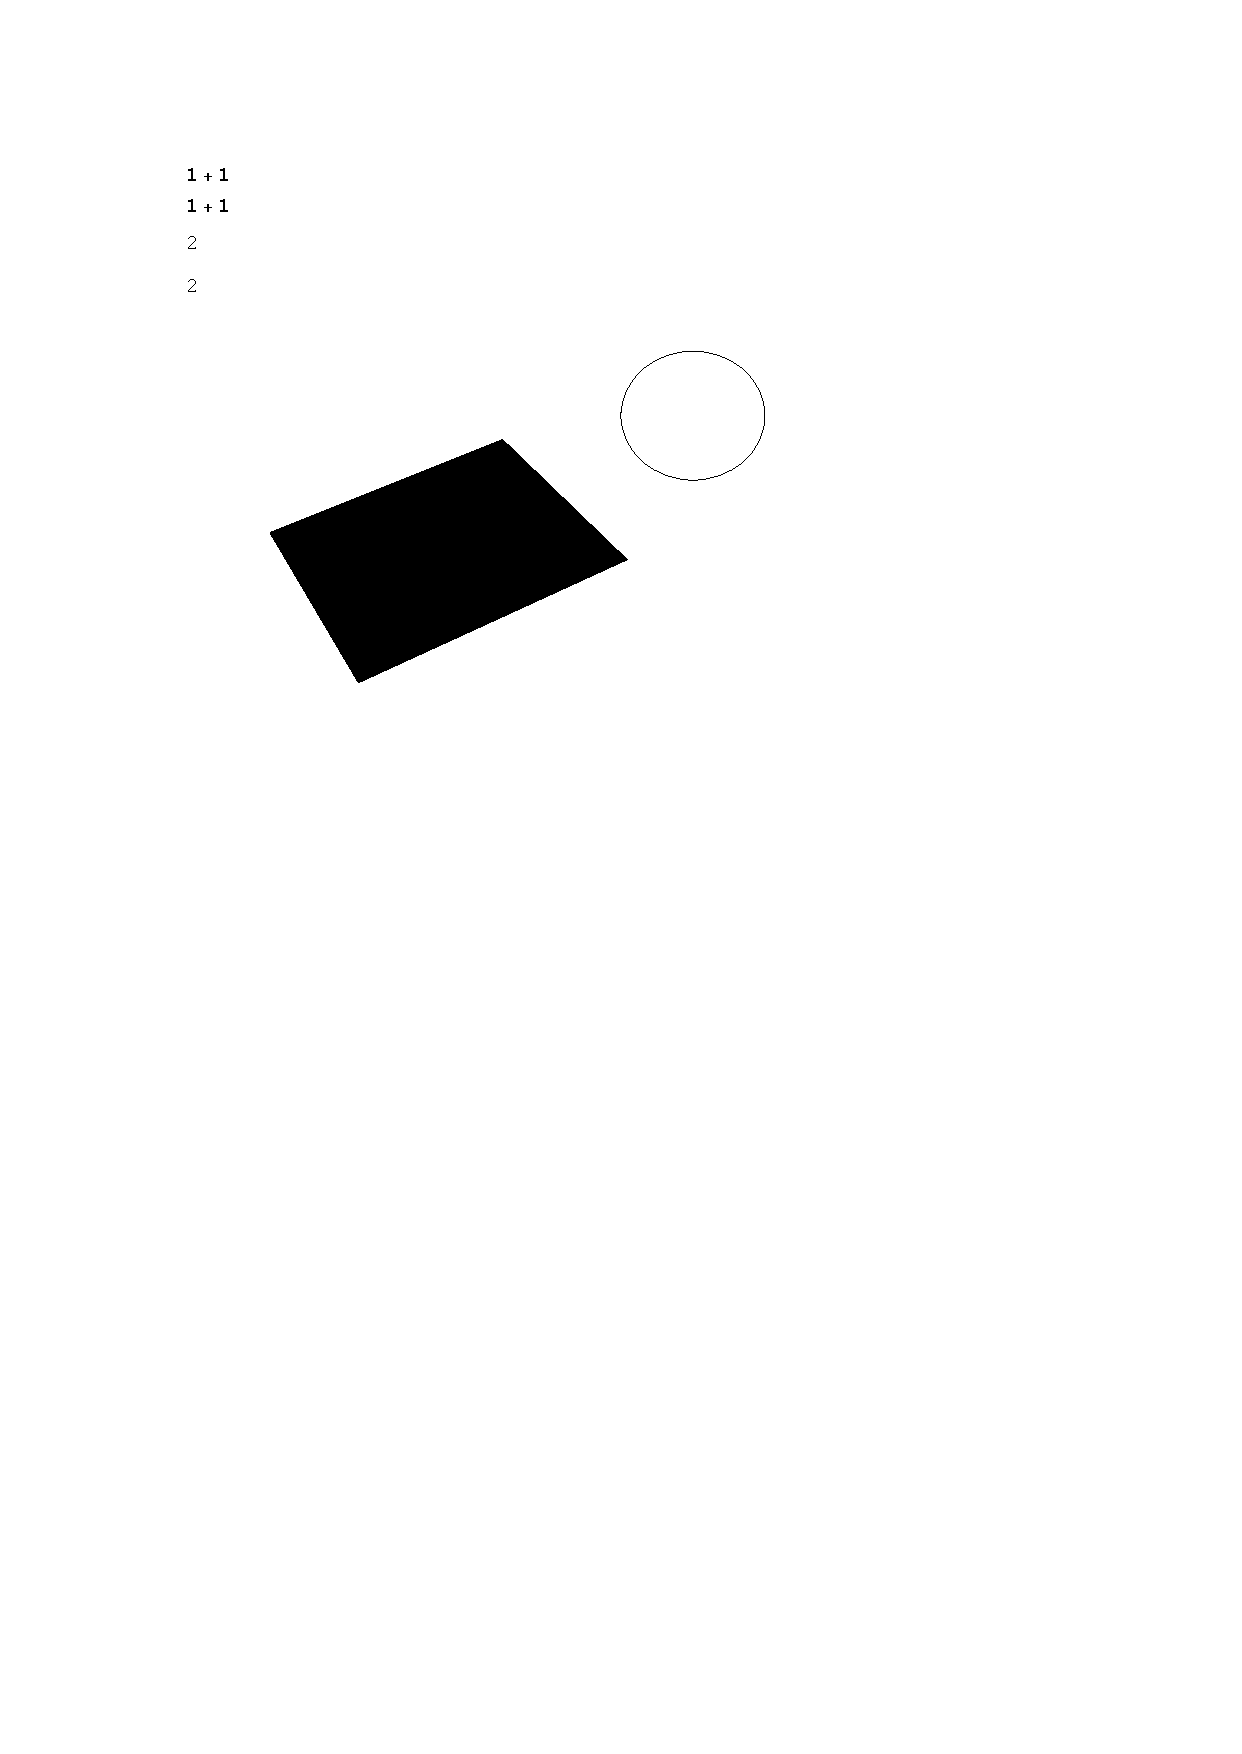
\includegraphics[width=12cm]{../Figures/1.pdf}
\caption{...}
\label{fig1}
\end{figure}

\end{document}